\sekshun{Rectangle Integration}
\label{Rectangle_Integration}
\index{rectangle integration}
\index{integration!rectangle}

The rectangle method computes an approximation to a 
definite integral by finding the area of a collection of rectangles whose heights are determined 
by the values of the function.  Specifically, the interval $[a,b]$ over which the function is to 
be integrated is divided into $N$ equal subintervals of length $h = (b-a)/N$. The rectangles are 
drawn with one base along the $x$-axis. Depending on whether the method is left, right, or midpoint,
the left corner, right corner, or midpoint, respectively, of the side opposite the base lies on the 
graph of the function. The approximation to the integral is 
then calculated by adding up the areas (base multiplied by height) of the $N$ rectangles, 
giving the formula:
\begin{equation}
\int_a^b f(x) dx \approx h \sum_{n=0}^{N-1} f(x_n) \label{eq:rectangle}
\end{equation}
where
\begin{equation}
  h=(b-a)/N  \label{eq:subinterval-width}
\end{equation}

The formula for $x_n$ for the left, right, and midpoint methods are given in Table \ref{tab:xn-rectangle}.
As $N$ gets larger, the rectangle method becomes more accurate. This is illustrated in the series of plots
in Figure \ref{fig:rectangle}.

\begin{table}[htbp]
\centering
\caption{Formula for $x_n$ in Equation \ref{eq:rectangle} of 
rectangle numerical integration methods.} 
\label{tab:xn-rectangle}
\begin{tabular}{cc}
\textbf{Method} & \textbf{$x_n$} \\ \toprule
left & $a+nh$ \\ \midrule
right & $a+(n+1)h$ \\ \midrule
midpoint & $a+\left(n + \frac{1}{2}\right)h$ \\ \bottomrule
\end{tabular}
\end{table}

\begin{figure}
\centering
\subcaptionbox{$N=4$}{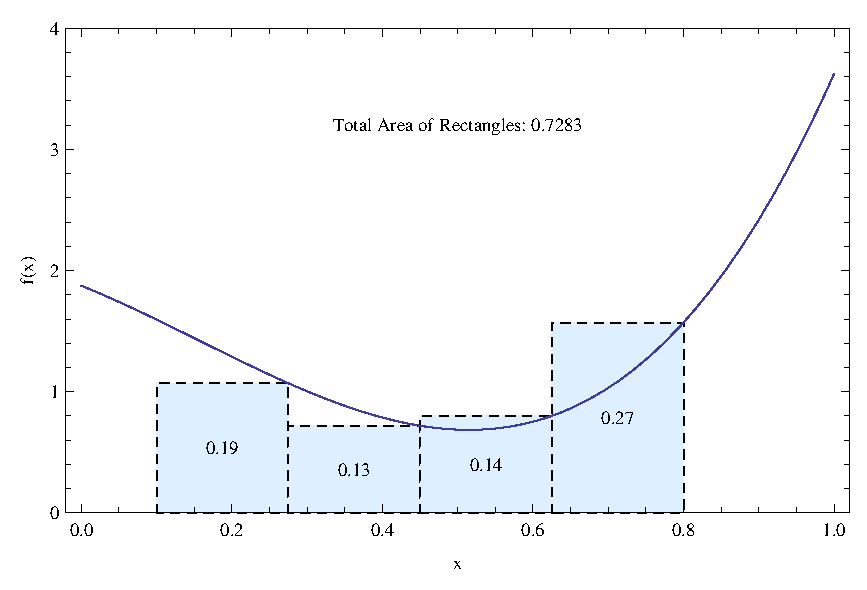
\includegraphics[scale=.6]{fig/rightrectangle-4.eps}}
\subcaptionbox{$N=6$}{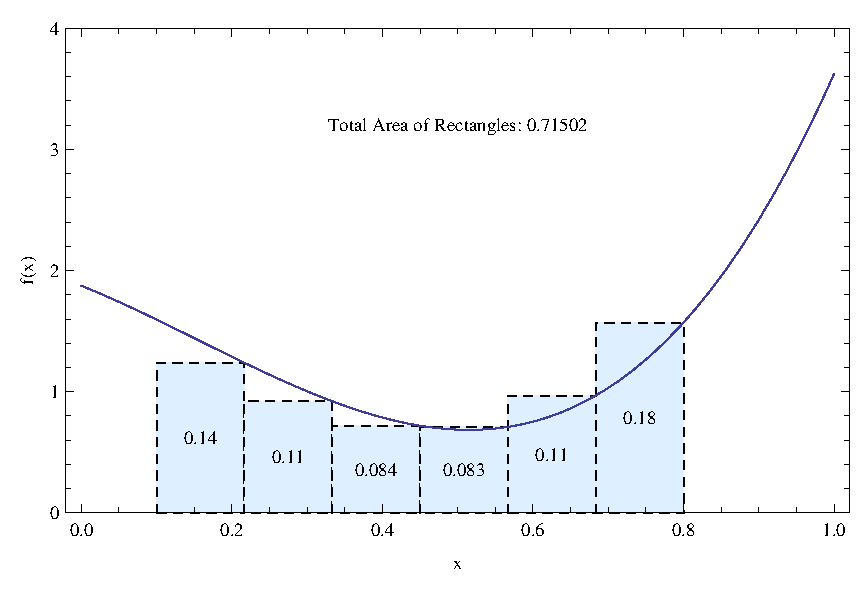
\includegraphics[scale=.6]{fig/rightrectangle-6.eps}}
\subcaptionbox{$N=10$}{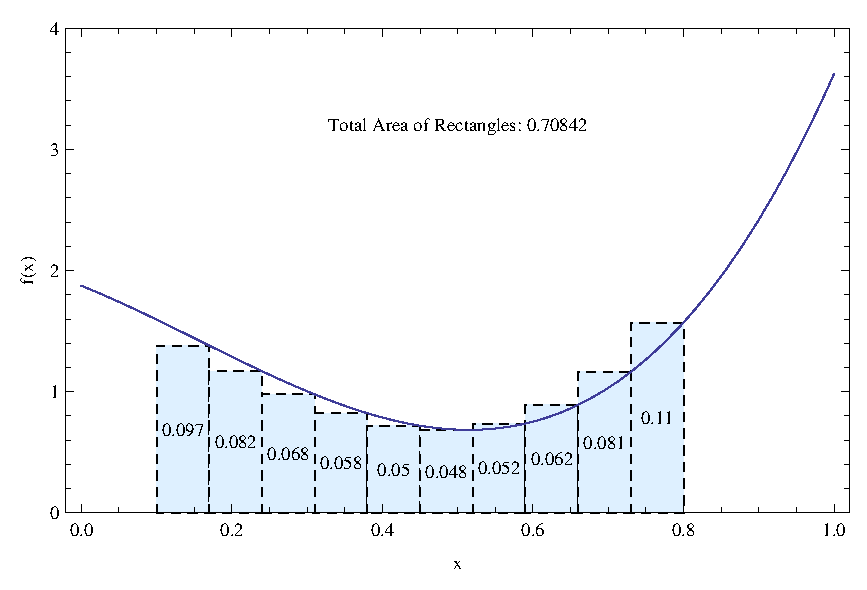
\includegraphics[scale=.6]{fig/rightrectangle-10.eps}}
\caption{Numerical integration of $f(x) = (2 x-0.5)^3+(1.5 x-1)^2-x+1$ for $x$ in $[0.1,0.8]$
by the (right) rectangle method for increasing values of $N$. The number inside each rectangle is
the area of that rectangle, and the total area is displayed on each graph.
The exact value of the integral is 0.70525.}\label{fig:rectangle}
\end{figure}

If $f(x)$ is increasing or decreasing on the interval $[a,b]$, the maximum error $E$ 
for left or right rectangular numerical integration is given by
\begin{equation}
E \leq \frac{b-a}{N}\left|f(b)-f(a)\right| \label{eq:lr-rectangle-max-error}
\end{equation}

We can create a helper function to compute the maximum error for left and right rectangle
methods using \ref{eq:lr-rectangle-max-error}. The calculated value will be used
in tests for the left and right rectangle methods to check that the result is within 
the maximum error expected for a given $a$, $b$, and $N$. 
\begin{enumspec}
\item\spec{1} Helper function \lstinline{leftRightRectangleMaxErr} returns the
maximum error expected for left or right rectangle method numerical integration. It 
takes in a reference to a pre-defined function $f$, the bounds $a$ (real) and $b$ (real) of the 
interval for definite integration, and the number $N$ (integer) of subintervals used.
The function will be entered in \lstinline{leftRightRectangleMaxErr.chpl}.
\meetsrequirement{5}
\end{enumspec}

\begin{chapelhelper}{leftRightRectangleMaxErr.chpl}
\begin{chapel}
proc leftRightRectangleMaxErr(a: real, b: real, N: int, f){
  return ((b-a)/N)*abs(f(b)-f(a));
}
\end{chapel}
\end{chapelhelper}

\begin{seamlessnote}
In \lstinline{seamless} vernacular, the helper files are chunks of code that are used to support
testing that the developer wants to have outside of the tests. The most likely reason being that
the code contains setup or auxiliary functions that are used for multiple tests. In our example
above, we are using some foresight and envisioning that the \lstinline{leftRightRectangleMaxErr}
function will also be used in a test for the left rectangle numerical integration function. To 
extract the helper files from your latex source files, run the following command in the same
directory as your latex source:
\begin{verbatim}
[./tutorial/] $ make helpers
\end{verbatim}
This command runs the \lstinline{helpers} target in the Makefile at the root of the 
tutorial directory (\lstinline{./tutorial/Makefile}. A Makefile is a text 
file written in a certain prescribed syntax. Together with the \lstinline{make} utility, it 
helps automate repetitive commandline tasks such as building software from its source files. 
In this case, the \lstinline{helpers} target cleans out the \lstinline{./tutorial/helper} directory and
executes the \lstinline{./util/extract\_helpers} python script with the appropriate arguments.
\end{seamlessnote}

One of the functions that we need to test our methods against is $f(x) = x^3$, 
with $a=0$, $b=1$, and $N=100$.
Since the function is increasing on the interval $[0,1]$, we can use 
the helper function that we just created to compute the maximum expected error. We are
ready to create our first test for a function that we will write to compute the definite
integral using the left rectangle method. This function will be called 
\lstinline{leftRectangleIntegration}
and will be written to \lstinline{leftRectangleIntegration.chpl}.
\begin{enumspec}
\item\spec{2}
Test \lstinline{leftRectangleIntegrationTest.chpl} loads modules
\lstinline{leftRightRectangleMaxErr} and
\lstinline{leftRectangleIntegration}.
It defines a function \lstinline{f} that takes $x$ (real) and returns $x^3$ (real).
It passes $a=0.0$, $b=1.0$, $N=100$, and \lstinline{f} to the function
\lstinline{leftRightRectangleMaxErr} and stores the result in the variable
\lstinline{maximumError} (real).
It passes $a=0.0$, $b=1.0$, $N=100$, and \lstinline{f} to the function
\lstinline{leftRectangleIntegration} and stores the result in the variable
\lstinline{calculated}.
Variable \lstinline{exact: real} is initialized with the exact value of the integral from
Mathematica, 0.25.
It then checks to see if the absolute value of the difference between \lstinline{calculated} 
and \lstinline{exact} is less than or equal to \lstinline{maximumError} and sets 
\lstinline{verified: bool}. The test writes out \lstinline{verified} and a passing
test results in \lstinline{true}.
\meetsrequirement{5.1}
\end{enumspec}

\begin{chapelexample}{leftRectangleIntegrationTest.chpl}
A test for \lstinline{leftRectangleIntegration}.
\begin{chapelpre}
\end{chapelpre}
\begin{chapel}
use leftRightRectangleMaxErr;
use leftRectangleIntegration;
proc f(x:real):real {
  return x**3;
} 
  
var calculated:real;
var exact:real = 0.25;  // from Mathematica
var maximumError:real = leftRightRectangleMaxErr(a = 0.0, b = 1.0, N = 100, f = f);
var verified:bool;

calculated = leftRectangleIntegration(a = 0.0, b = 1.0, N = 100, f = f);
verified = (abs(calculated - exact) <= maximumError);
writeln(verified);
\end{chapel}
\begin{chapelpost}
\end{chapelpost}
\begin{chapeloutput}
true
\end{chapeloutput}
\end{chapelexample}

\begin{seamlessnote}
Now that we have our first test, we need to extract it from the latex source and verify
that it does not pass.
To extract the test from the latex source and run it:
\begin{verbatim}
[./tutorial/] $ make tests
[./tutorial/] $ make test
\end{verbatim}
These commands run the \lstinline{tests} and \lstinline{test} targets in the same Makefile referenced above.
In this case, the \lstinline{tests} target cleans out the \lstinline{./tutorial/test} directory and
executes the \lstinline{./util/extract_tests} python script with the appropriate arguments.
The \lstinline{test} target changes to the \lstinline{./tutorial/test} directory and 
executes the \lstinline{start_test} csh script that comes with
the chapel distribution (in \lstinline{CHPL_HOME/util}). The script compiles and executes each of the
chapel source files in the test directory 
(\eg \lstinline{leftRectangleIntegrationTest.chpl} as in the example above) 
and compares the output with the contents of a file with a \lstinline{.good} extension
(\eg \lstinline{leftRectangleIntegrationTest.good} for the above test). 
\end{seamlessnote}
\begin{TODO}
  Update test target to extract all code and run tests.
\end{TODO}

The code that provides the \lstinline{leftRectangleIntegration} function is straightforward.
\begin{enumspec}
\item\spec{3} Function \lstinline{leftRectangleIntegration}, for an interval
  of integration, $[a,b]$,
  takes the left end value of the interval, \lstinline{a: real}, the right end value
  of the interval, \lstinline{b: real}, the number of subintervals for the numerical
  integration, \lstinline{N: int}, and the function to be integrated, \lstinline{f}.
  The function stores the width of the subinterval calculated from Equation 
  \ref{eq:subinterval-width} in the variable \lstinline{h: real}. It initializes the variable
  \lstinline{sum: real} to zero, and for each value of $n$ in the summation of Equation~\ref{eq:rectangle},
  it computes \lstinline{x_n: real} according to the expression in Table~\ref{tab:xn-rectangle} and adds
  the value of \lstinline{f(x_n)} to \lstinline{sum: real}. The function returns the product of 
  \lstinline{sum: real} and the subinterval width, \lstinline{h: real}.
  \meetsrequirement{1}
\end{enumspec}

\begin{chapelsource}{leftRectangleIntegration.chpl}
\begin{chapel}
proc leftRectangleIntegration(a: real(64), b: real(64), N: int(64), f): real(64){
  var h: real(64) = (b - a)/N; 
  var sum: real(64) = 0.0;
  var x_n: real(64);
  for n in 0..N-1 {
    x_n = a + n * h;
    sum = sum + f(x_n);
  }
  return h * sum;
}
\end{chapel}
\end{chapelsource}

\begin{seamlessnote}
  We can now verify that test \lstinline{leftRectangleIntegrationTest.chpl} passes. First
  we need to extract the chapel source from our latex file and then run the test that was
  written previously:
\begin{verbatim}
[./tutorial/] $ make sources
[./tutorial/] $ make test
\end{verbatim}
These commands run the \lstinline{sources} and \lstinline{test} targets in our Makefile.
In this case, the \lstinline{sources} target cleans out the \lstinline{./tutorial/source} directory and
executes the \lstinline{./util/extract_sources} python script with the appropriate arguments, putting
the source code that we've defined in our latex file into the \lstinline{./tutorial/source} directory.
\end{seamlessnote}

\begin{TODO}
  Describe refactoring of the above code.
\end{TODO}

For a function $f$ which is twice differentiable, the maximum error $E$ is given by
the following equation:
\begin{equation}
E \leq \frac{(b-a)h^2}{24} f''(\xi) \label{eq:rectangle-max-error}
\end{equation}
for some $\xi$ in $[a,b]$.

Create a helper function to compute the maximum error:
\begin{chapelhelper}{midpointRectangularIntegrationMaximumError.chpl}
\begin{chapel}
proc midpointRectangularIntegrationMaximumError(a: real, b: real, N: int, fppxi){
  var h:real = (b-a)/N;
  return ((b-a)*h**2/24) * fppxi;
}
\end{chapel}
\end{chapelhelper}
